\section{Basin estimation}\label{sec:certificates}

This section bounds the basin of the forced orbit from inside, at three levels of modelling that must be kept apart:\label{sec:cert-levels} a circle criterion for the delay equation of the averaged, linear-force model (Section~\ref{sec:cert-global}); linear matrix inequalities, numerically verified, for finite-dimensional collocation models of the averaged (C2) and the time-periodic (C3) delay equation (Section~\ref{sec:cert-model}); and the simulator, with the time-periodic force, loss of contact and the surface memory, which checks both (Section~\ref{sec:cert-c2}). No statement is made here for the physical machine.

\subsection{Global attractivity below the uncontrolled limit}\label{sec:cert-global}

Let the forced orbit be unclipped, $\lvert b(t)\rvert\le\Vmax$. In the averaged model the deviation $\tilde x=x-x_p$ obeys Eq.~\eqref{eq:dev} below with $aH(t)$ replaced by its mean $\overline{aH}$, and its command is $\sat_{\Vmax}(b-g\dot{\tilde x})-b=-\varphi(t,g\dot{\tilde x})$, where
\begin{equation}\label{eq:phi-sector}
  \varphi(t,y)=b(t)-\sat_{\Vmax}\bigl(b(t)-y\bigr),\qquad 0\le\varphi(t,y)\,y\le y^2 ,
\end{equation}
a time-varying nonlinearity in the sector $[0,1]$, for deviations of any size. With the feedback removed, the map from $-\varphi$ to $y=g\dot{\tilde x}$ is
\begin{equation}\label{eq:Ls}
  L(s)=\frac{g\,s\,G_a(s)\,G(s)}{1-\overline{aH}\,\bigl(1-e^{-sT}\bigr)\,G(s)} ,
\end{equation}
the uncontrolled cut with the actuator, whose characteristic roots lie in the open left half-plane for $a<\alim(0)$.

\begin{proposition}[Global attractivity]\label{prop:circle}
Let $a<\alim(0)$, $\lvert b(t)\rvert\le\Vmax$ for all $t$, and $\mu=\inf_{\omega\in\mathbb R}\operatorname{Re}\bigl[1+L(i\omega)\bigr]>0$. Then every solution of the averaged, linear-force delay model with the clipped DVF law converges to the forced orbit.
\end{proposition}

The proof (Supplementary Material, Section~\ref{S-supp:std-proofs}) applies the circle criterion \citep{zames1966inputII,desoer1975feedback}. Let $a_{\mathrm{circ}}(n,g)$ be the largest depth below $\alim(0)$ up to which the condition holds and the forced orbit is unclipped. At the scheduled gains of Section~\ref{sec:feasibility}, the forced orbit of the averaged delay model attracts every solution up to $(1-10^{-3})\,a_{\mathrm{circ}}$ at all 251 speeds, with the frequency condition proved on the whole frequency axis by interval arithmetic and the unclipped forced orbit checked on a dense depth grid (Supplementary Material, Sections~\ref{S-supp:circle} and~\ref{S-supp:std-circle}). The median of $a_{\mathrm{circ}}$ over the speeds is $0.967\,\alim(0)$; it lies below $0.9\,\alim(0)$ at 78 of the 251 speeds.
% src (interval proof): verification/paper/circle_interval.py/.json (251 speeds verified at (1 - 1e-3) a_circ, 0 undecided boxes); circle_interval.log
% src: verification/paper/circle_criterion.json (g_best: ratio_eff_median 0.9667; n_ratio_eff_below_0p9 78)

\subsection{Collocation model and LMI conditions}\label{sec:cert-model}\label{sec:cert-lmi}

For $\lvert b(t)\rvert<\Vmax$, the deviation $\tilde x$ obeys
\begin{equation}\label{eq:dev}
\begin{aligned}
&m\ddot{\tilde x}+c\dot{\tilde x}+k\tilde x=aH(t)\,\big[\tilde x(t)-\tilde x(t-T)\big]+K_a\ddot{\tilde q},\\
&\ddot{\tilde q}+2\zeta_a\omega_a\dot{\tilde q}+\omega_a^2\tilde q=\sat_{\Vmax}\!\big(b(t)-g\dot{\tilde x}\big)-b(t),
\end{aligned}
\end{equation}
where $\tilde q$ is the deviation of the actuator coordinate of Eq.~\eqref{eq:eom} and $aH(t)$ the coefficient of Eq.~\eqref{eq:aHt}. C2 replaces $aH(t)$ by its mean $\overline{aH}$, Eq.~\eqref{eq:aHmean}; C3 keeps it. The history $\tilde x(t+\vartheta)$, $\vartheta\in[-T,0]$, is collocated at $N=16+4\lceil T\omega_n/2\pi\rceil$ (20--32) Chebyshev nodes $\vartheta_j$ \citep{breda2005pseudospectral,breda2015book}. With $\xi=\big[\tilde x,\ \dot{\tilde x},\ \tilde q,\ \dot{\tilde q},\ \tilde x(t+\vartheta_1),\dots,\tilde x(t+\vartheta_N)\big]^\top\in\mathbb R^{4+N}$,
\begin{equation}\label{eq:coll}
\dot\xi=\mathcal A(t)\,\xi-B\,\psi(k^\top\xi,t),\qquad \mathcal A(t)=A_0+Bk^\top+aH(t)\,E_r,
\end{equation}
with the feedback row $k^\top=-g\,e_2^\top$ ($k$ is not the stiffness here), $E_r=\big(e_2e_1^\top-e_2e_{4+N}^\top\big)/m$, $e_i$ the unit vectors, and $A_0$, $B$ in Supplementary Material, Eq.~\eqref{S-eq:app-A0}. The clip enters only through the dead zone
\begin{equation}\label{eq:deadzone}
\psi(w,t)=w-\sat_{\Vmax}\!\big(b(t)+w\big)+b(t),
\end{equation}
which, unlike that of a fixed saturation, moves with the forced command.
% src: README §12.2; src/c2_certificate.py (model, nodes_for, history_nodes); src/c3_periodic.py (model)

\begin{lemma}[Moving dead zone]\label{lem:sector}
If $\bar b\ge\sup_t\lvert b(t)\rvert$ and $u_0=\Vmax-\bar b>0$, then for all $t$, $w$ and $v$
\begin{equation}\label{eq:sector}
\lvert w-v\rvert\le u_0\quad\Longrightarrow\quad\psi(w,t)\,\big[\psi(w,t)-v\big]\le0 .
\end{equation}
\end{lemma}

Equation~\eqref{eq:sector} is the generalised sector condition of \citet{gomesdasilva2005antiwindup} for the moving dead zone. With $v=\Gamma\xi$ for a free row $\Gamma$, $\mathcal V(\xi)=\xi^\top P\xi$, $\mathcal E(P)=\{\xi:\mathcal V(\xi)\le1\}$, $W=P^{-1}$, $Y=\Gamma W$ and a scalar $S>0$, the inverse of the S-procedure multiplier \citep{tarbouriech2009antiwindup,tarbouriech2011book}, the conditions read
\begin{gather}
\begin{bmatrix}-(\mathcal AW+W\mathcal A^\top)-2\lambda W & BS-Y^\top\\ SB^\top-Y & 2S\end{bmatrix}\succ0, \label{eq:lmi-dec}\\
\begin{bmatrix}W & Wk-Y^\top\\ k^\top W-Y & u_0^2\end{bmatrix}\succeq0, \label{eq:lmi-incl}\\
\begin{bmatrix}W & W\chi^\top\\ \chi W & (\delta f_z)^2\end{bmatrix}\succeq0,\qquad \chi=e_1^\top-e_{4+N}^\top,\quad \delta=0.5, \label{eq:lmi-valid}\\
\begin{bmatrix}1 & \beta e^\top\\ \beta e & W\end{bmatrix}\succeq0, \label{eq:lmi-size}
\end{gather}
with a decay margin $\lambda\ge0$ and a direction $e$ along which the size $\beta$ is maximised. For $e=e_2$, $\beta$ is a certified kick in m/s; for $e=-\xi_p(0)$, minus the orbit state at $t=0$ with its history, $\beta\ge1$ certifies the step entry at the entry phase of the simulator.

\begin{proposition}[Averaged model, C2]\label{prop:c2}
Let $\mathcal A$ be constant, $\bar b$ and $u_0$ as in Lemma~\ref{lem:sector}, and $W\succ0$, $Y$ and $S>0$ satisfy Eqs.~\eqref{eq:lmi-dec}--\eqref{eq:lmi-valid} with $\lambda=0$. Then, for Eq.~\eqref{eq:coll} with the dead zone~\eqref{eq:deadzone}, $\mathcal E(W^{-1})$ is forward invariant from every phase, every trajectory starting in it converges exponentially to the forced orbit, and $\lvert x-x(t-T)\rvert\le\delta f_z$ along it. If Eq.~\eqref{eq:lmi-size} also holds, $\beta e\in\mathcal E(W^{-1})$.
\end{proposition}

Both proofs are in Supplementary Material, Section~\ref{S-supp:std-proofs}. The validity bound~\eqref{eq:lmi-valid} excludes gross loss of contact. With the memoryless part of the loss of contact as a second sector nonlinearity, the certified kick falls by 6--\SI{15}{\percent} at 0.5 and $0.9\alim$ at the four speeds of Section~\ref{sec:bistab-basin}, and at $0.98\alim$ no certificate exists, so near the limit the estimates rest on the linear force law (Supplementary Material, Section~\ref{S-supp:std-contact}).
% src: verification/paper/contact_sector.py/.json (ratio beta2/beta1 at 0.5 a_lim 0.937/0.878/0.937/0.930 and at 0.9 a_lim 0.851/0.877/0.902/0.930 (1090/1420/2500/2870 rpm); at 0.98 a_lim beta2 = 0)

\subsection{Results}\label{sec:cert-c2}

\label{sec:cert-check}Every candidate $(W,Y,S)$ returned by the solver was checked independently at $\lambda=0$, in floating point rather than by interval arithmetic (Supplementary Material, Section~\ref{S-app:lmi}). C2 was computed at the 48 clipped points of Section~\ref{sec:bistability} (Fig.~\ref{fig:cert}); all 48 passed the check. Wherever the simulated critical kick is finite (29 points), $\beta$ lies below it, by factors $\Delta v^*/\beta$ of 1.5--28 and with a median of 2.3 from $0.7\alim$ upwards. Boundary points of the ellipsoid in 18 sampled directions (off-axis runs), applied in the simulator, never ended in chatter (3456 runs; Table~\ref{S-tab:cert}). The critical kick of the averaged collocation model is itself 0.62--0.99 times $\Delta v^*$ (median 0.92), so the gap lies mainly between the certificate and its own model. Doubling $N$ changes $\beta$ by $-5.0$ to $+0.6$\,\% at ten of eleven points (Table~\ref{S-tab:nconv}). The step entry is certified only at $0.3\alim$ at three of the four speeds, never at productive depths.
% src: src/c2_certificate.py (scaling, lmi, check, certify); src/c3_periodic.py (check); README §12.3
% src: README §12.4; results/c2_validate.npz, c2_summary.json (validate), c3_summary.json (errata.c2_validate: 1.48-27.59, median 2.34 from 0.7 a_lim); results/c2_validate.npz recomputed: td_min infinite at 19 points; model/TD 0.620-0.989, median 0.92; offaxis 0/3456
% src: verification/paper/certs_nconv_summary.py/certs_nconv.json (summary: n_points 11, n_with_2N 10, rel_2N_min -0.0496 at 1090 rpm 0.5 a_lim, rel_2N_max +0.0063 at 2870 rpm 0.5 a_lim)
% src: README §12.5; results/c2_step.npz, c2_summary.json (step), c3_summary.json (errata.c2_step: 1.48/1.61/1.04 corrected at 0.3 a_lim; 0.16-0.72 at 0.5-0.9 a_lim)

\begin{figure}[!tbp]
\centering
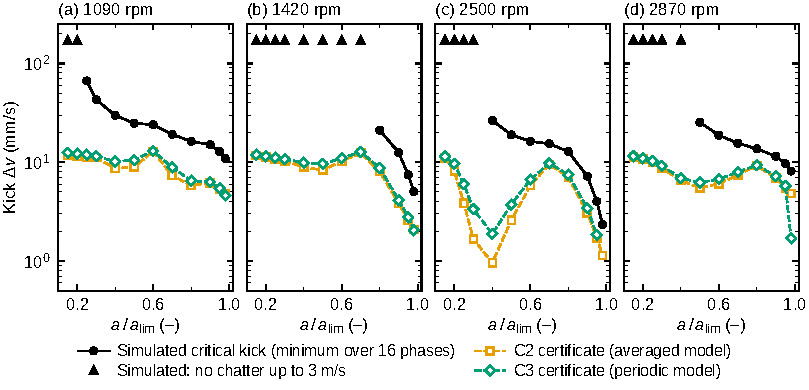
\includegraphics[width=\textwidth]{figures/fig06_certificates.pdf}
\caption{Certified kick on the averaged model (C2, squares; command bound corrected as in Supplementary Material, Section~\ref{S-supp:std-bound}) and on the periodic model (C3, diamonds; valid at every phase) against the simulated critical kick $\Delta v^*$ (circles; minimum over 16 phases) at the speeds, depths and gain of Fig.~\ref{fig:basin}. Triangles: no chatter for any kick up to \SI{3}{\metre\per\second}. C3 is missing at \SI{2500}{\rpm} and $0.98\alim$, where no candidate passed the check.}
\label{fig:cert}
\end{figure}
% src: README §12.4; results/c2_validate.npz, c2_summary.json (validate)

\label{sec:cert-periodic}\label{sec:cert-c3}The periodic certificate C3, with $W(t)$ and $Y(t)$ linear in time on $M=16$ segments of the tooth period (Supplementary Material, Proposition~\ref{S-prop:c3}), passed the check at 47 of the 48 points; no off-axis run from its boundary ended in chatter. As the critical kick of the periodic model is 0.97--1.05 times that of the averaged model, the factor of about 2.3 between the certificates and the simulated basin near the limit is not caused by averaging (Supplementary Material, Section~\ref{S-supp:std-c3}).
% src: README §14.1, §14.2; src/c3_periodic.py (aH, orbit, enclosure)
% src: README §14.5, §14.6; results/c3_basin.npz, c3_summary.json (basin)
% src: README §14.5, §14.7, §14.10; results/c3_basin.npz, c3_summary.json (basin: phase_cert_below_td 448/448, phase_cert_below_model 688/688, offaxis 0/3384, td_over_cert_from_07, periodic_over_averaged_model 0.9727-1.0516)
